% Import Packages
\documentclass[12pt]{article}
\usepackage[utf8]{inputenc}
\usepackage[table]{xcolor}
\usepackage{listings}
\usepackage[letterpaper, margin=1in]{geometry}
\usepackage{graphicx}
\usepackage{verbatim}
\usepackage{underscore}
\usepackage{fancyhdr}
\usepackage{hyperref}
\usepackage{enumitem}
\usepackage{hanging}
\usepackage{seqsplit}
\usepackage{multirow}
\usepackage{multicol}
\usepackage{array}
\usepackage{longtable}
\usepackage{xurl}

% Command for quick and easy bibliography
\newcommand\hangingindent[1]{\begin{hangparas}{0.5in}{1} #1 \end{hangparas}\vspace{0.5cm}}

% Command for coloring a table cell light gray and emboldening the text
\newcommand\cellhead[1]{\cellcolor{lightgray}\textbf{ #1 }}

% Change the color of hyperlinks to blue
\renewcommand\UrlFont{\color{blue}}

\pagestyle{fancy}
\fancyhf{}
\fancyhead[R]{Wall Guys: Final Report}
\fancyhead[L]{}
\fancyfoot[C]{\thepage}

\begin{document}

    \begin{titlepage}
        \begin{center}
            \vspace*{1cm}
            \Huge\textbf{ECE 397: Final Report}

                \vspace{0.5cm}
                \LARGE Wallcopter Project
    
            \vspace{1.5cm}
            \textbf{Team 13: Wall Guys}

                \vspace{0.5cm}
                Tien Dao, Hardik Goel, Sarthak Hans, Jaden Mossman, and Anand Pudi

                \Large
                Sponsor: Dr Ahmet Enis Cetin

                Instructor: Dr Matthew Alonso

                \LARGE

            \vfill             
            \includegraphics[width=0.4\textwidth]{resources/uic_logo.png}

            % ASSIGNMENT DESCRIPTION
            \vspace{0.8cm}
            University of Illinois Chicago\\
            Spring 2023
                
        \end{center}
    \end{titlepage}

    \tableofcontents

    \newpage
    \section{Abstract}
        High rise buildings and the undersides of bridges are important structures that need to be examined for safety purposes, but this is often a difficult task as they are hard to reach places and typically experience high wind.
        Even when reached, the unstable environment often causes the resulting images used for inspections to be blurry and difficult to analyze.
        The aim of the project was to identify an accessible drone platform, modify it for inspections, and maintain control to collect data with the drone at typical heights and environmental conditions.
        The drone has an additional attachment that includes a camera and sensors that will assist the drone in taking pictures.
        Additionally, there are slide attachments atop the drone, which allow it to make contact with the upper surface and remain stable.
        All of these factors together allow us to obtain a stable image used for inspections.
        The captured images will be sent to a receiving computer, where an image-detecting algorithm will detect any cracks or damages.
        We have used the DJI Tello and ESP 32 microcontroller for the project and have included additional prop guards to allow the drone to ceilings periodically.
        Our accomplishments include successfully designing and building the drone prototype, incorporating the necessary components, and testing its functionality in stable flight.
        After inspecting some nearby structures we were able to test the range and image quality of the pictures providing a cost-effective solution to structural engineers and those responsible for ensuring the safety of these structures.
        This inspection run can be found with the videos that we recorded.
    
    \newpage
    \section{Overview}

        \subsection{Project Goals}
            The aim of this project is to develop an attachment onto a drone to allow additional features for inspection purposes.
            These inspections will be done in hard to reach places like under bridges or high rise buildings.
            We are looking to make at least a prototype that can go up to the ceilings of most areas and can navigate via a wireless control system.
            Our priority is as follows: main focus on functionality, producing a minimum working prototype, and then try to reduce the cost of the drone itself if possible.

        \subsection{Needs Statement}
            High rise buildings and the undersides of bridges are important structures that need to be examined for safety purposes, but this is often a difficult task as they are hard to reach places and typically windy and tough environments.
            Drones are often deployed to conduct these examinations, but there are limitations to their performance when coming into close contact with those surfaces.
            Another limitation is the lack of stable connection when the drone is a certain distance away from the user.
            These limitations, among others, provide a challenge to the autonomous examination of bridges and buildings.

        \subsection{Objective Statement}
            The objective of this project is the design of a drone that is able to navigate in a stable manner while remaining its set distance to the ceiling or object it is touching.
            The drone will have a camera installed that can capture images or give live feed for inspection purposes.
            Sensors will be used in order to calculate and articulate the distance between the drone and the ceiling.
            Standard wireless communication will be through the microcontroller that allows the user to control the device from a distance.

        \newpage
        \subsection{Background}
            \begin{enumerate}[label=\Alph*.]
                \item The basic concept that lays behind this wall-copter relies on the control system that keeps the copter stable to prevent collision or unintended side effect when approaching ceilings or walls.
                The current limitation lies on the unintended shifts of the blade speed when the copter gets too close to the wall's surface. 
                The other factor is the difficulty of control when the drone gets too close to such a surface.
                Surprisingly, there don't seem to be any current remedies that exist in the market right now, so we do not have a way to compare our project to it.
                Still, there are current market competitors who offer drones with strong frames that are used for inspections using LiDAR mapping technology.
                Those drones, whoever do not approach the ceilings or navigate close to the effect of rotors being sucked into a surface.
                They have to remain within a distance of 1.5 times the size of the rotor from the upper wall to remain safe and stable [1].
                There are other approaches to keeping the drone stable within these areas as there are studies focused on navigation via tilting the drone against the wall in order to ascend in a stable manner [2].
                This research focuses on scaling vertically using the Tilt Motor Mechanism that results in some successes in keeping the drone stabilized enough for certain tasks.
                An existing prototype exists for that research, but it does not seem like they have a focus on releasing that product into the market [2].
                One other alternative approach done by students from Shandong University of Science and Technology suggests creating a drone that would stick to walls/ceilings similar to geckos [4].
                This particular design focuses on solving the problem of inspection when natural disasters occur, which is only similar to our objective, but the designs would be very beneficial to keep in mind.
                Once again, this is only a test product, not meant for release in the market and would not be our direct competitor.
                
                \indent Upon further background research, we found out that a license would be required in order to fly certain types of drone [5].
                Luckily, a license is not required for small indoor drones that are used for commercial purposes.
                So initial testing using indoor labs will not require such a license but will be different for outdoor tests.
                When looking into the drone market, typical drone prices vary quite a bit, from a very cheap price of \$30 that can go up to thousands [6].
                Usually the bigger the drone and more functionality it offers, the more expensive the product will be.
                So in order to remain competitive, our drone need to be within a reasonable range of around \$100-\$250, the amount that our budget would be allocated.
                
                \item Our background of this project is very clear from the beginning since it's a sponsored project, we still interviewed the professor to answer more questions we had.
                From this, we understand that the professor wants a product that currently does have strong competitors within the market space. 
                \begin{enumerate}[label=\roman*.]
                    \item Functionality: The goal is to make a drone which navigates in high places without the current problems (shaking, height limit close to ceiling, stability).
                    \item Appearance: It will look just like a common drone that currently exists in the market except with add-ons that would assist it with our goal.
                    \item Cost: The cost of the drone is preferred to be as low as possible since it is a commercial product.
                    For now our goal is just your standard drone cost that one can find for a reasonable price range of 40-100 dollars.
                    \item User Interface: Our user interface would be that of your standard drone control, but with potentially an extra set of control for the sets of wheels that will be at the top of the device.
                    \item Reliability: We want to obtain a product that will be consistent with every use.
                    This device should be very reliable since it builds upon the existing frame of a normal drone.
                    \item Power Requirements: The drone runs on a standard rechargeable battery which can also power our wheel system. Perhaps additional modification might be required if there is more power required to run the drone, but currently it would be safe to assume a standard drone battery would be able to run just fine also.
                    \item Expected Product Lifetime: As this kind of drone would be more difficult to navigate, we can assume it has a lower average product lifetime.
                    However, with proper use and care, it should still last only a little bit less if not the same amount of time as a standard drone.
                    \item Interfacing requirements with other systems.
                    \item User training needs: It is safe to assume that there will be a learning curve to the device in addition to learning how to navigate using the extra set of wheels on top.
                    Such a process can be learned just like a normal drone and should still be able to learn with some time and effort.
                    \item Government regulations and licensing: According to Part 107 of the FAA, any drone that weights over 250g needs to be registered even if it's only for commercial purposes.
                    This process shouldn't be too difficult and there isn't too much of a barrier to obtain one for use.
                    \item Industry standards: We follow the rules given to all drones.
                    Since our product is newer, we don't know what other standards might be applied to it.
                    So currently we'll be abiding by the current drone industry standards.
                    \item Safety issues: The drone has the issue of crashing into high terrains and falling onto passerby below.
                    There is also potential that objects that the wheels made contact with on the ceiling could potentially break and fall.
                    The device has the same safety problems as normal drones, only with additional unforeseen safety issues that come with driving it on the wall/ceiling.
                    \item Environmental Concerns: This device should be fairly safe environmentally to operate, with a low carbon footprint.
                    There are still concerns that when it crashes or is lost, if not recovered, it would be non-biodegradable as it is made out of plastics and other electronic components.
                    The battery that is used to operate the drone is also bad for the environment if not recycled correctly.
                \end{enumerate}
            \end{enumerate}
        \newpage

        \subsection{Marketing Requirements}
            For our marketing requirements, we focus on the standard requirements that most drones have.
            Additionally, we consider its cost-effectiveness along with the development cost of our design when making our requirements.
            We also include data from the interview that we had with our sponsor when making considerations of our marketing requirements.
            \begin{enumerate}[label=\arabic*.]
                \item The wall-copter must be able to climb on flat surfaces.
                \item The wall-copter should be stable.
                \item The wall-copter should be easy to use.
                \item The wall-copter should be cost-effective and easy to maintain.
                \item The wall-copter must be able to be controlled by a user from a distance.
                \item The wall-copter should be able to operate within a reasonable amount of time.
                \item The wall-copter should have minimal environmental impact.
                \item The wall-copter should follow proper regulations policies.
            \end{enumerate}
        
        \subsection{Objective Tree}
            There were many considerations when it came to our Objective Tree, we decided that there should be a split focus among maneuverability and stability, which both had high percentages.
            The ease of use would come as an extra priority in order to make it easier for our users to operate.
            The diagram below shows all the sub-focuses and their priority within each category.
            \centerline{\Large \underline{\textbf{Wall Copter}}}
            \begin{multicols}{3}
                \noindent Traversing Ceilings /

                \noindent\underline{Rough Surfaces 0.45}
                
                \noindent Walls 0.10
                
                \noindent Ceilings 0.70
                
                \noindent Underneath bridges 0.20

                \columnbreak

                \noindent\underline{Ease of Use 0.10}

                \noindent Limited controls 0.36

                \noindent Long operating time 0.64

                \columnbreak
                
                \noindent\underline{Be Stable 0.45}
                
                \noindent Sturdy structure 0.42
                
                \noindent Accurate motion sensors 0.35
                
                \noindent Long-lasting motors 0.23

            \end{multicols}
        
        \subsection{Additional Information}
            Upon further research, we found additional inspection drones that are available in the market [8].
            Those, however, are all very expensive as they are high-end drones that are usually manufactured for very specific tasks and are not flexible for its high price.
            On the high side of this, we have drones like the AscTec Falcon 8 that go up to \$48,000 in the market [9].
            Even on the low side, drones like the DJI Inspire 2 would still go up to \$3,299 [10].
            From this research, we also noted that there have yet to be any drones in the market with an elliptical ski design.
    
    \newpage
    \section{Engineering Requirements / Technical Specifications}
        \begin{longtable}{ | m{4.25cm} | m{5cm}| m{5.4cm} | }
            \hline
            Marketing Requirement & Engineering Requirement & Justification \\\hline
            1,2 &
            The wall-copter should be able to go to the heights of the ceiling, usually around at 20ft. &
            The product should adhere to the drone standard of being airworthiness (IEEE 1936.1-2021) \\\hline
            2 &
            The wall-copter should have standard drone speed of around 20 mph tops. &
            The device should be able to meet mechanical, and electrical requirements (IEEE 1937.1-2020) \\\hline
            4 &
            The device should be within a reasonable price range of around \$100-\$250. &
            Although there isn't a requirement for prices, the device should follow standards for estimating costs (IEEE 3001.4-2020)\\\hline
            6 &
            The wall-copter should be able to run for at least 10-15 minutes and is rechargeable. &
            The battery should follow IEEE guidelines for safety and usability (IEEE 1625-2008)\\\hline
            7 &
            The device should not emit any pollution and should not affect its surrounding environment too much. &
            The device should be following all the standards and remain environmentally sustainable (IEEE 1680.1) \\\hline
            3,5 &
            Users should be able to follow FAA regulations when operating the drone. &
            The user needs to be properly taught to operate the wall-copter in order to be safe for themselves and others (IEEE 1936.1-2021) \\\hline
            8 &
            The user needs to have the proper license needed in order to operate the device. &
            Qualification of operator is needed in order to use the product (IEEE 1936.1-2021) \\\hline
            4 &
            The drone blades and parts such as batteries and microcontroller/ sensors should be easily disconnected in order to clean/replace. &
            The device have to adhere to proper functionality for easy maintenance (IEEE 1937.1-2020) \\\hline
            4 &
            The wall-copter should be easy to make with additional modification to a standard drone production. &
            The product needs to be in line with manufacturing process control (IEEE 1625-2008) \\\hline
            1,2,3 &
            The wall-copter should be able to perform all tasks while maintaining a good lifespan of 150-800 flight hours. &
            The device should be very reliable in order for repeated use (IEEE 1680.1) \\\hline
            3,5 (including user interface) &
            The user should be able to operate the device after some basic training similar to how a normal drone should operate. &
            As the product require data to be collected for operations, it should also follow the drone data classification (IEEE 1936.1-2021) \\\hline
        \end{longtable}

        \subsection{Non-Applicable Parameters}
            \subsubsection*{Political}    
                There isn't a current political aspect to our device as it is something that is used for inspection purposes.
                The only potential aspect would come from the privacy concerns that might come from the use of the drone for its unintended reason.
                That is something that every kind of drone would have by default.
                Since the locations our drone is made to inspect is hard reach in nature, we do not expect there to be any privacy issues.

            \subsubsection*{Social and Cultural}
                Our drone does not have any social and cultural features that would fit as an engineering requirement.
                Its uses are only intended for technical reasons and should not have any social related issues or any form of cultural influence.
    
    \newpage
    \section{Engineering Design Alternatives}
        \subsection{Design 1}
            This design includes an ultrasonic sensor in order to determine the distance between the drone and the ceiling/objects.
            We would have ball bearing wheels at the top in various selected locations.
            The drone would handle the movement both vertically and horizontally.
            In order to control the drone, we would be using a controller that communicates with the drone.
            The drone still would include a camera on top for image capturing.

            \vspace{0.5in}
            \centerline{\includegraphics{./resources/assignment3-Design1.schematic.drawio.pdf}}

            \vspace{0.5in}
            \begin{tabular}{|c|l|}
                \hline
                \multicolumn{2}{|c|}{\textbf{Design 1, Level 0}} \\\hline
                Module & Wall-Copter \\\hline
                \multirow{3}{3cm}{Inputs}
                    & - Power: Lithium-ion Battery\\
                    & - User Input by Controller \\
                    & - Sensor Data (Ultrasonic Sensor) \\
                    \hline
                \multirow{2}{3cm}{Outputs}
                    & - Drone Movement \\
                    & - Image Data Capturing \\
                    \hline
                \multirow{3}{3cm}{Functionality}
                    & - Precision flight control close to the roof through sensor data. \\
                    & - Movement along the roof with simple ball bearing wheels. \\
                    & - Capturing image for building inspections. \\
                    \hline
                
            \end{tabular}
            
        \newpage
        \subsection{Design 2}
            Using the idea of having two cameras (one on top, one built in) with an imaging system that would be used to determine the distance to the wall.
            Will use motorized wheels on top of the drone for horizontal navigation.
            
            \vspace{0.5in}
            \centerline{\includegraphics{./resources/assignment3-Design2.schematic.drawio.pdf}}

            \vspace{0.5in}
            \begin{tabular}{|c|l|}
                \hline
                \multicolumn{2}{|c|}{\textbf{Design 1, Level 0}} \\\hline
                Module & Wall-Copter \\\hline
                \multirow{3}{3cm}{Inputs}
                    & - Power: Lithium-ion Battery\\
                    & - User Input by Phone App \\
                    & - Imaging Data \\
                    \hline
                \multirow{3}{3cm}{Outputs}
                    & - Drone Movement \\
                    & - Wheel Movement \\
                    & - Image Data \& Video \\
                    \hline
                \multirow{4}{3cm}{Functionality}
                    & - Precision flight control close to the roof. \\
                    & - Capturing images and using them for computer vision flight control. \\
                    & - Live feedback of data through Wi-Fi. \\
                    & - Navigation on the roof through motorized wheels. \\
                    \hline
                
            \end{tabular}

        \newpage
        \subsection{Design 3}
            This design uses lasers placed in triangular configuration to triangulate the correct distance between the drone and the ceiling.
            It will also be using some kind of ski device to assist in movement at the ceiling or rough surfaces.
            The drone will also be controlled by a standard controller that comes with the product.

            \vspace{0.5in}
            \centerline{\includegraphics{./resources/assignment3-Design3.schematic.drawio.pdf}}

            \vspace{0.5in}
            \begin{tabular}{|c|l|}
                \hline
                \multicolumn{2}{|c|}{\textbf{Design 1, Level 0}} \\\hline
                Module & Wall-Copter \\\hline
                \multirow{3}{3cm}{Inputs}
                    & - Power: Lithium-ion Battery\\
                    & - User Input by Controller \\
                    & - Laser Sensors \\
                    \hline
                \multirow{2}{3cm}{Outputs}
                    & - Drone Movement \\
                    & - Image Data Capturing \\
                    \hline
                \multirow{3}{3cm}{Functionality}
                    & - Using sensor data for stabilized flight control close to the roof. \\
                    & - Capturing image for building inspections. \\
                    & - Using ski design to help device navigate at the top. \\
                    \hline
                
            \end{tabular}
            \newpage

        \subsection{Differences and Similarities Between Designs}
            Our three designs are very similar in principle as they all have the goal of detecting when the drone is close to the ceiling and giving feedback to the system.
            The designs were built upon this principle, keeping the drone from hitting the ceiling.
            They also have ways in which they navigate while touching the ceiling.
            They all share a control system in which we communicate to it through a controller, what we usually see in standard drones.
            Although these designs are similar, they are quite different as we try to create variations that can hopefully determine the best outcome.
            Their main differences are the sensors that go on them.
            Design 1 uses an ultrasonic sensor while Design 2 uses a camera with imaging processing and Design 3 uses lasers.
            Each of these variations have their own strengths and weaknesses that vary with costs.
            However, they all achieve the same goal of telling the drone if there's an object overtop of it (and how close) in order to avoid collision.
            Another difference is how the drone is going to navigate over the ceiling, with Design 1 using ball bearing wheels that would just serve as a way to move while Design 3 uses skis in order to slide while the drone itself performs the movement.
            In that case, movement will be handled by the drone itself, reducing the design complexity.
            Design 2 uses motorized wheels, which runs using its own motor, this will allow the drone to move without compromising its vertical movements.
            One last difference is how they are controlled, all would have the same communications via Wi-Fi with the main difference being that Design 1 and Design 3 using a standard drone controller, while Design 2 aims to use a phone app as its control.

    \newpage
    \section{Selection of Best Alternative Design}
        % TODO come back to this section, Tien made some changes I need to spend more time unpacking
        \subsection{Design Criteria}
            \begin{enumerate}
                \item \textbf{Development Cost}
                
                One of the main restrictions to a project, the amount of materials and the quality of the materials itself depend on this figure.
                We take our budget into consideration when comparing our development cost with other criteria.

                \item \textbf{The Group's Technical Knowledge about the Design Alternative}
                
                We are limited by what we and our advisor can cover with their expertise.
                The general goal is to keep it to something we can learn and realistically execute.
                Technical knowledge that is too complex to execute should be placed lower in priority.

                \item \textbf{Time Needed to Complete Design and Development}
                
                We should always keep our time limit in mind when it comes to making a design.
                Being mindful of our time limit is crucial for us to effectively achieve our goals.
                In this case, it is the end of the semester.

                \item \textbf{Suitability for Demo for 397}
                
                We should aim to get a prototype for our demonstration, so choose a design that is reasonable for making a prototype.
                Our prototype should be functional or at least most of it should be done for presentation within the expo.

                \item \textbf{Ease of Product Use}
                
                A product should always be easy to use or at least fairly achievable after minimal training in order to gain interests from the consumer.
                Keeping things in the lower side of the complexion will aid in usability and increase interest in the use of our product.
            \end{enumerate}

        \subsection{Pair-wise Comparison of Criteria}
            \begin{center}\begin{tabular}{|l|l|l|l|l|l|}
                \hline
                & \cellhead{Tien} & \cellhead{Jaden} & \cellhead{Anand} & \cellhead{Hardik} & \cellhead{Average} \\\hline
                \cellhead{Dev Cost} & 0.274 & 0.067 & 0.215 & 0.2 & 0.189 \\\hline
                \cellhead{Knowledge} & 0.251 & 0.325 & 0.110 & 0.2 & 0.222 \\\hline
                \cellhead{Time Needed} & 0.298 & 0.222 & 0.311 & 0.2 & 0.258 \\\hline
                \cellhead{Demo} & 0.093 & 0.313 & 0.185 & 0.2 & 0.198 \\\hline
                \cellhead{Ease of Use} & 0.083 & 0.072 & 0.179 & 0.2 & 0.133 \\\hline
            \end{tabular}\end{center}
        
        \subsection{Design Alternatives Relative to Criteria}
            \begin{center}\begin{tabular}{|l|r|c|c|c|}
                \hline
                \cellhead{Criteria} & \cellhead{Avg Weight} & \cellhead{Design 1} & \cellhead{Design 2} & \cellhead{Design 3} \\\hline
                \cellhead{Dev Cost} & 0.189 & 4 & 2 & 3 \\\hline
                \cellhead{Knowledge} & 0.222 & 3 & 2 & 3 \\\hline
                \cellhead{Time Needed} & 0.258 & 4 & 2 & 3 \\\hline
                \cellhead{Demo} & 0.198 & 1 & 5 & 3 \\\hline
                \cellhead{Ease of Use} & 0.133 & 2 & 3 & 3 \\\hline      
                    & \cellhead{Score:} & 2.917 & 2.727 & 3 \\\hline
            \end{tabular}\end{center}
        
        \subsection{Final Decision Matrix}
            \noindent For additional tables, see Appendix D.

            \begin{center}\begin{tabular}{|l|r|r|r|r|}
                \hline
                \cellhead{Criteria} & \cellhead{Avg Weight} & \cellhead{Design 1} & \cellhead{Design 2} & \cellhead{Design 3} \\\hline
                \cellhead{Dev Cost} & 0.189 & 4 & 2 & 3 \\\hline
                \cellhead{Knowledge}& 0.222 & 3 & 2 & 3 \\\hline
                \cellhead{Time Needed} & 0.258 & 4 & 2 & 3 \\\hline
                \cellhead{Demo} & 0.198 & 1 & 5 & 3 \\\hline
                \cellhead{Ease of Use} & 0.133 & 2 & 3 & 3 \\\hline
                & \cellhead{Score:} & 2.917 & 2.727 & 3 \\\hline
            \end{tabular}\end{center}
        
        \subsection{Final Decision}
            After collecting the data from each member, we obtained a personalized comparison of each of our criteria.
            These data were then analyzed to obtain the geometric mean and weights.
            We then compare these data in a pair-wise comparison table and get an average of our weights.
            This way, we know what the team thinks of each criteria overall, with Time Needed being the highest weight at 0.257 and knowledge coming second at 0.22.
            We then proceed with giving a score to all criteria based on the design as a group.
            Finally, we input the data into our Final Decision Matrix.
            To our expectation, design 3 has the highest score of 3 after all the calculations.
            What surprised us was how close design 2 is to winning, with the score being 2.92.
            It would also mean there are certain factors of design 2 that seem to work out within our criteria.
            After some analysis, we try to understand what is good and will be incorporating it into our design 3 for the best overall results.
            This design features lasers as our sensors and wheels overtop that seems to fit most of our preference, we will also be attempting to incorporate the demo capability of design 2 into it to improve our final design.

    \newpage
    \section{Preliminary Design}
        \subsection{Level 1 Schematic}
            \centerline{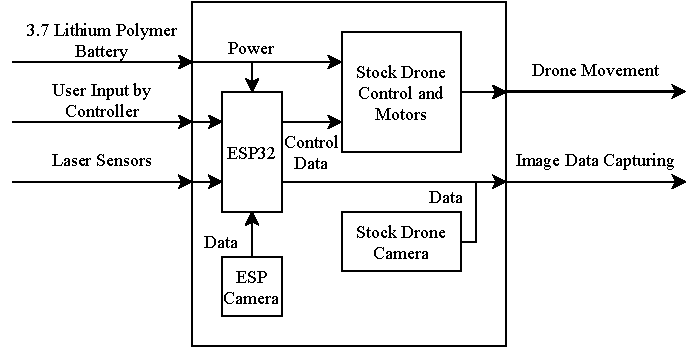
\includegraphics{./resources/level1.pdf}}
        \subsection{Circuit Diagram}
            \centerline{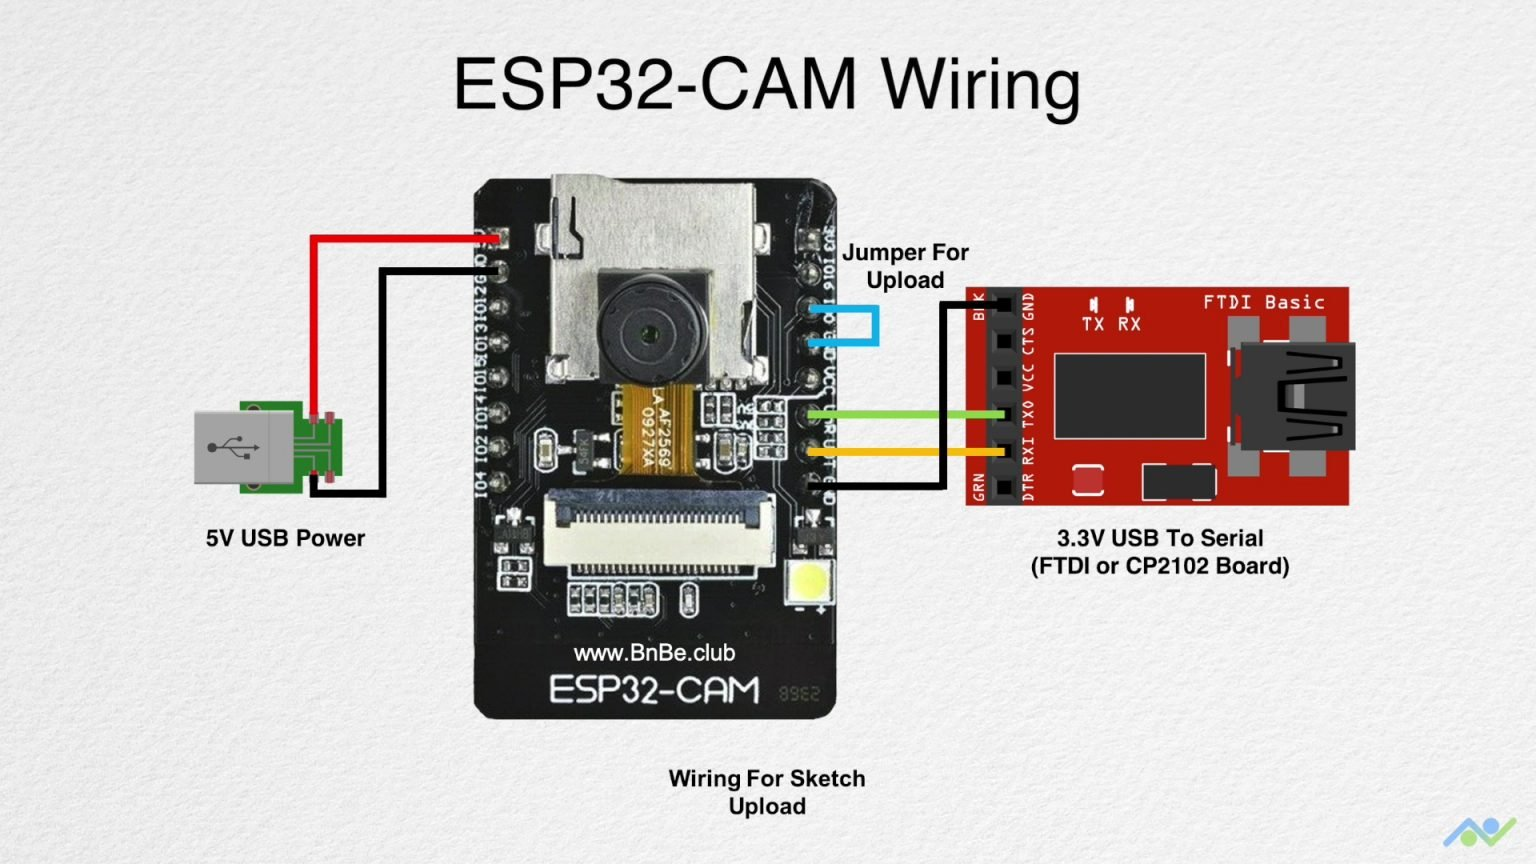
\includegraphics[width=0.4\textwidth]{resources/esp32cam_wiring.jpg}}
        % \subsection{Software Design}
        % TODO add software diagram or get rid of this subsection
    
    \newpage
    \section{Testing}
        \subsection*{Testing and Data}
            Our group performed multiple tests in order to figure out the carry capacity of the Tello drone.
            In our test, we used all the coins that the team could find as a weight to test (dime, pennies, and quarter).
            We put all the coins into a ziplock bag and taped it at the bottom of the drone.
            As we progressed through the many different versions, we stopped using the coin bag and used the actual add-on devices that were originally intended for the drone.
            Our prototype designs also observed many test flights, which we won't include every flight due to the sheer amount of tests we did.
            We will, however, include the most notable tests that we performed with meaningful or notable takeaways.

            \subsubsection*{Data}
            \begin{longtable}{ | m{1.5cm} | m{2cm}| m{3cm} | m{4cm} | m{4cm} |}
                \hline
                Test \# & Condition & Test Load & Result & Note \\\hline

                1 & Indoor &
                Full bag of coins &
                Drone flew but didn't remain long in the air &
                Failure might be due to the weight imbalance \\\hline

                2 & Indoor &
                Fewer coins &
                Drone flew but is very unstable in the flight pattern &
                The swinging of the bag is the cause for such instability \\\hline

                3 & Indoor &
                ESP-32 (10g) &
                Stable flight &
                Landing was not good due to the sensors at the bottom being obstructed by the ESP-32 \\\hline

                4 & Indoor &
                Stack of coins (55-60g) &
                Stable flight &
                Drone flew and maintained its balance in a stable manner. The drone overheated very quickly afterwards \\\hline

                5 & Indoor &
                No test load &
                Successful flight &
                Nothing much to note as we were testing out our control system using the computer \\\hline

                6 & Indoor &
                Basket version 1 along with ESP and ToF &
                Flight observed but crashed after little time in the air &
                The drone managed to lift off but could not maintain balance in the air. The lead to a crash as the drone swayed. \\\hline

                7 & Indoor &
                Tello frame &
                Stable flight but crashed right after the drone touched the ceiling &
                The drone flew in a stable manner, but once we tested out the ceiling touch, the frame would touch the propeller and crash the drone. \\\hline

                8 & Indoor &
                Slide and ski design &
                Stable flight, some stable ceiling navigation but crash after some movement &
                Similar to previous test, drone crashed due to the skis touching the propeller \\\hline

                9 & Indoor &
                Second basket design &
                Failure to lift off &
                The drone could not fly after multiple attempts \\\hline

                10 & Indoor &
                Third basket design &
                Successful flight along with ceiling navigation &
                Very smooth navigation with great ceiling movements. Landing was successful. \\\hline

                11 & Indoor &
                Third basket design with the ESP and ToF board &
                Lift off but could not remain in the air for long &
                Battery needed to be at full capacity to handle the heavy load. Drone is quick to overheat \\\hline

                12 & Indoor &
                Fourth basket design with all the components &
                Successful flight with some minor stability issues &
                The drone flew very well but had very minor balancing issues and leaned to one side \\\hline

            \end{longtable}

            \newpage

            \subsubsection*{Conclusions}
                \newcommand{\teststatement}[3]{
                    \vspace{0.5cm}\noindent\textbf{#1} (#2) - #3
                }

                \teststatement{Test 1} {All the coins and ziplock bag taped at the bottom} {
                    The drone flew but did not remain in the air and would tumble down due to the weight imbalance.
                    The team concluded the bad weight distribution to be the major factor that caused the failure.
                }

                \teststatement{Test 2} {Tying wire onto the drone and hanging the ziplock bag} {
                    With the full amount of weight, the drone was still not able to fly in a stable manner.
                    However, after we removed a lot of the coins, the drone flew.
                    One thing to note is the swinging caused by the ziplock bag caused the drone to not have difficulty following commands.
                }

                \teststatement{Test 3} {Flying with the ESP-32 tapped into the drone} {
                    Something to note is the problem of when the ESP-32 is taped on top of the Tello, the wings would be interfered with, preventing flight.
                    The group decided to tape the ESP-32 at the bottom instead.
                    The drone is observed to fly in a stable manner and there doesn't seem to be that much problem with it.
                }

                \teststatement{Test 4} {Coin stack at the payload limit of 60g taped directly on top of the drone} {
                    The drone flew with good balance, navigating the way we intended.
                    It was quick to overheat since some of the heat vents were taped over, preventing the drone from cooling effectively.
                }

                \teststatement{Test 5} {Testing using a computer as the control system} {
                    The test was successful, the control was seamless.
                    We managed to control the drone the same way that the Tello app can.
                }

                \teststatement{Test 6} {Using our first basket design we put the ESP and ToF on it then taped the basket to the bottom of the drone} {
                    The result was unsuccessful, the drone could not fly when there was too much weight.
                    When it managed to fly, balancing was a major issue leading to an eventual failure as we could not control the drone.
                    Another thing to note is that the drone overheated even faster than test 5 as the heat vents were blocked by the basket.
                }

                \teststatement{Test 7} {Test using the Tello frame} {
                    This test's purpose was due to our consideration of using either the Tello frame or our slide design for ceiling navigation.
                    The frame was lightweight enough to help sustain a stable flight but failed when it comes to navigating on the ceiling.
                    This is due to the frame's flexibility, it would bend and interfere with the propellers.
                }

                \teststatement{Test 8} {Test using the ski design} {
                    We observe a stable flight similar to the previous test, but the drone crashes in a similar manner as the pins holding the skis touch the propeller.
                    The takeaway from the test is that there should be a bridge in between the skis to provide some structural stability.
                }

                \teststatement{Test 9} {Second basket design along with the ESP and ToF} {
                    The drone could not lift off due to the imbalance in the weight design.
                    We tried many attempts even with adding extra coins on one end to try to offset the balance issue.
                    All of these showed no results as the drone failed to lift off far past the ground.
                }

                \teststatement{Test 10} {Flying with third basket design} {
                    This is our most successful flight with meaningful results so far.
                    We had a successful lift off and landing along with great ceiling navigation.
                    One thing to note is that the skis seem to need to be taller to allow more room for the ESP camera.
                }

                \teststatement{Test 11} {Flying with the third basket along with the ESP, ToF, Boost Converter, and battery} {
                    The drone lifted off the first attempt but could not fly any higher.
                    Subsequent attempts also failed to produce a liftoff as the drone was not at full battery.
                    In a different day's test, the drone could fly at full battery but could only remain in the air for around 5-8 seconds.
                }

                \teststatement{Test 12} {Fourth basket along with all the components} {
                    In this test, we did not try to confirm the ceiling maneuverability as the location that we tested in had a very high ceiling, and we were not comfortable in trying to move around on the ceiling.
                    The drone lifted off successfully and could move around in a fairly stable manner.
                    We did, however, observe some slight off balance issue when flying it and worked to try to rebalance the drone.
                }
    
    \newpage
    \section{Final Design}
        \noindent Wiring schematic:

        \centerline{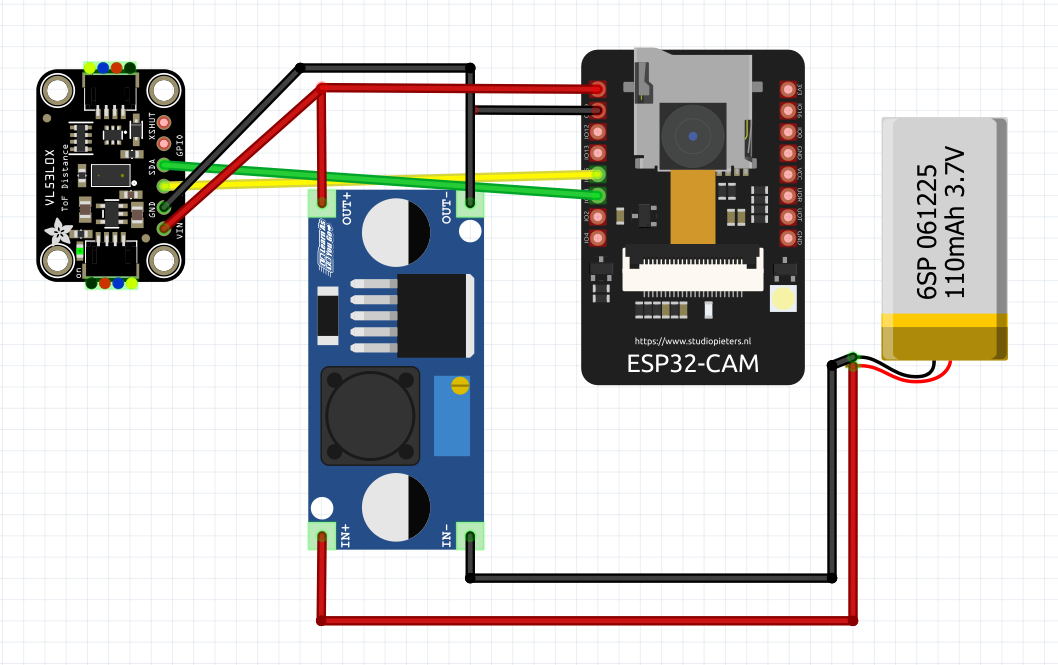
\includegraphics[width=0.7\textwidth]{./resources/wiring_schematic.png}}

        \vspace{2cm}\noindent Solidworks model of skis:

        \centerline{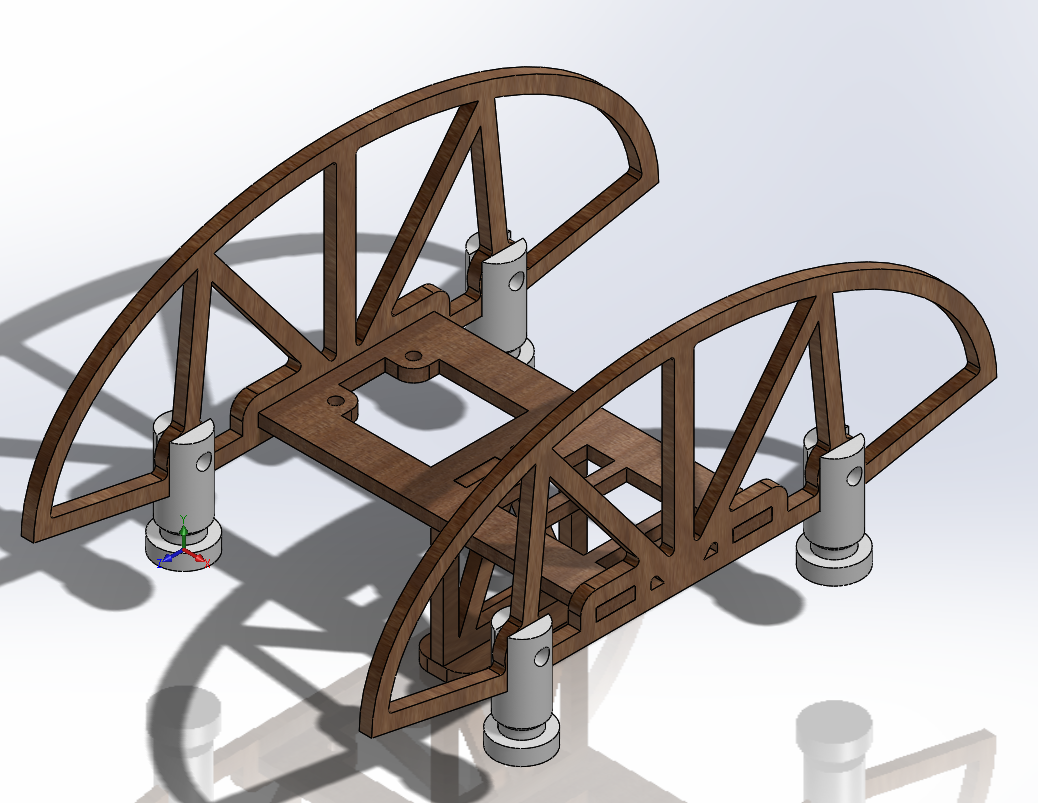
\includegraphics[width=0.7\textwidth]{./resources/basket_final_solidworks.png}}

        \vspace{2cm}\noindent Solidworks models of pins:

        \centerline{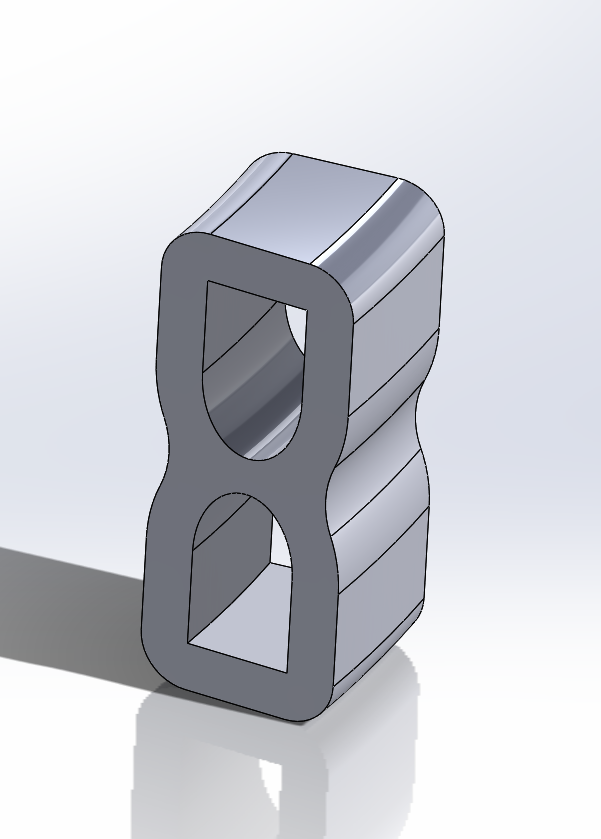
\includegraphics[width=0.7\textwidth]{./resources/propguard_clip.png}}

        \vspace{2cm}\noindent Diagram of communication system:

        % TODO: Better diagram
        \centerline{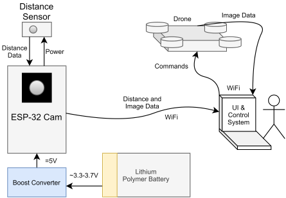
\includegraphics[width=0.7\textwidth]{./resources/comm_diagram.png}}

        \newpage
        \subsection{Budget}
            This budget is made based on all the materials that were needed for the drone project.
            Due to some difficulties buying drones from the approved vendors, the group decided to pay out of pocket for some products like the Drone, ESP-32, and the ToF sensor.
            Their cost will all be included in the report, along with the items that the group obtained from the vendors.
            \begin{tabular}{|l|r|r|r|}
                \hline
                Item & Price (\$) & Amount & Cost (\$) \\\hline
                Tello Drone & 100 & 1 & 100 \\\hline
                Tello Drone (Amazon) & 110 & 1 & 110 \\\hline
                TOF10120 & 4.5 & 1 & 25 \\\hline
                ESP-32 & 10 & 1 & 10 \\\hline
                Back up propellers & 5 & 2 & 15 \\\hline
                & & & \\\hline
                & & Total cost (\$) & 264.5 \\\hline
            \end{tabular}
    
    \newpage
    \section{Task Allocation and Timeline}
        \subsection*{Week 2}
            \subsubsection*{Tien Dao}
                \begin{itemize}
                    \item Research 3 viable drone options and purchase a drone
                    \item Email Professor Cetin and schedule bi-weekly meetings
                \end{itemize}
            \subsubsection*{Hardik Goel}
                \begin{itemize}
                    \item Research 3 viable wheel options
                    \item Research ways to mount ESP and wheels on a drone
                \end{itemize}
            \subsubsection*{Sarthak Hans}
                Joined team later in the semester
            \subsubsection*{Jaden Mossman}
                \begin{itemize}
                    \item Research 3 viable drone options and purchase a drone
                    \item Research how to interface an ESP-32 with a drone
                \end{itemize}
            \subsubsection*{Anand Pudi}
                \begin{itemize}
                    \item Research 3 viable wheel options
                    \item Research essential libraries for ESP-32 WiFi, Bluetooth, and motor control
                \end{itemize}
        
        \subsection*{Week 3}
            \subsubsection*{Tien Dao}
                \begin{itemize}
                    \item Budget for the drone, microcontroller, and wheels. Itemized list.
                \end{itemize}
            \subsubsection*{Hardik Goel}
                \begin{itemize}
                    \item Research about optimal drone payload including control system and wheels. Excel doc of data.
                \end{itemize}
            \subsubsection*{Sarthak Hans}
                Joined team later in the semester
            \subsubsection*{Jaden Mossman}
                \begin{itemize}
                    \item Updating google doc and previous report. PDF of report.
                    \item Reach out to EDT and ask about borrowing drone. Itemized list.
                \end{itemize}
            \subsubsection*{Anand Pudi}
                \begin{itemize}
                    \item Research ESP-32 WiFi, Bluetooth, and motor control libraries.
                \end{itemize}
        \subsection*{Week 4}
            \subsubsection*{Tien Dao}
                \begin{itemize}
                    \item Budget for the drone, microcontroller, and wheels. Itemized list.
                \end{itemize}
            \subsubsection*{Hardik Goel}
                \begin{itemize}
                    \item Research optimal drone payload including control system and wheels.
                    \item Design ideas for 3D printed mount as per Tello's design perspective.
                \end{itemize}
            \subsubsection*{Sarthak Hans}
                \begin{itemize}
                    \item Power distribution. Estimate time of flight total including the drone and the microcontroller on board.
                \end{itemize}
            \subsubsection*{Jaden Mossman}
                \begin{itemize}
                    \item Outline ESP code and create a Git repo with outlined code.
                    \item Update Google Doc and previous report.
                \end{itemize}
            \subsubsection*{Anand Pudi}
                \begin{itemize}
                    \item Budget for the drone, microcontroller, and wheels. Itemized list.
                \end{itemize}
        
        \subsection*{Week 5}
            \subsubsection*{Tien Dao}
                \begin{itemize}
                    \item Budget - Create an itemized list for the drone, microcontroller, and wheels.
                \end{itemize}
            \subsubsection*{Hardik Goel}
                \begin{itemize}
                    \item Design ideas for 3D printed mount - Design the ideal mount for the MCU, VL53L0X sensor, and wheels as per Tello's design perspective
                    \item Finalize communication scheme - Speak with Professor Paprotny about how to best route communications through devices and make a final decision on the communication scheme.
                \end{itemize}
            \subsubsection*{Sarthak Hans}
                \begin{itemize}
                    \item Power distribution - Develop a clear understanding of the power distribution between the Tello Drone and the ESP32 utilizing a voltage regulator.
                \end{itemize}
            \subsubsection*{Jaden Mossman}
                \begin{itemize}
                    \item Outline ESP and application code - Create a Git repo with outlined application code.
                    \item Finalize communication scheme - Speak with Professor Paprotny about how to best route communications through devices and make a final decision on the communication scheme.
                \end{itemize}
            \subsubsection*{Anand Pudi}
                \begin{itemize}
                    \item Purchase drone and supplies - Purchase an extra drone, extra propellers, and batteries from Best Buy through school form.
                \end{itemize}
            \subsubsection*{Team}
                \begin{itemize}
                    \item Meet in person to discuss progress and next steps.
                \end{itemize}
        
        \subsection*{Week 6}
            \subsubsection*{Tien Dao}
                \begin{itemize}
                    \item Research a complete drone build with parts. Create an itemized list of drone parts.
                \end{itemize}
            \subsubsection*{Hardik Goel}
                \begin{itemize}
                    \item Design ideas for 3D printed mount as per Tello's design perspective. Create an ideal mount for the MCU, VL530X sensor, and wheels.
                \end{itemize}
            \subsubsection*{Sarthak Hans}
                \begin{itemize}
                    \item Power distribution. Test the power distribution between the Tello drone and ESP32.
                \end{itemize}
            \subsubsection*{Jaden Mossman}
                \begin{itemize}
                    \item Outline application code. Create a git repo with outline code.
                \end{itemize}
            \subsubsection*{Anand Pudi}
                \begin{itemize}
                    \item Research a complete drone build with parts. Create an itemized list of drone parts.
                \end{itemize}
            \subsubsection*{Team}
                \begin{itemize}
                    \item Attend in person meeting
                \end{itemize}

        \subsection*{Week 7}
            \subsubsection*{Tien Dao}
                \begin{itemize}
                    \item Test the flight with attached ESP, sensor, and foam. Actual payload capacity.
                \end{itemize}
            \subsubsection*{Hardik Goel}
                \begin{itemize}
                    \item Make a ski mechanism for drone to glide on the ceiling. A lighter alternative to wheels.
                \end{itemize}
            \subsubsection*{Sarthak Hans}
                \begin{itemize}
                    \item Testing the power distribution between the Tello and ESP. A power distribution schematic.
                \end{itemize}
            \subsubsection*{Jaden Mossman}
                \begin{itemize}
                    \item Get ESP to send video straight to desktop app. Code outline.
                \end{itemize}
            \subsubsection*{Anand Pudi}
                \begin{itemize}
                    \item Find an alternative to Tello, in case the current scenario doesn't work. A second drone.
                \end{itemize}
            \subsubsection*{Team}
                \begin{itemize}
                    \item Attend in person meeting
                \end{itemize}
        
        \subsection*{Week 8}
            \subsubsection*{Tien Dao}
                \begin{itemize}
                    \item Review and update the team document and budget, taking into account any changes or new developments.
                \end{itemize}
            \subsubsection*{Hardik Goel}
                \begin{itemize}
                    \item Finalize and test the 3D model and mount for the propeller's propguard. Conduct necessary modifications if needed.
                \end{itemize}
            \subsubsection*{Sarthak Hans}
                \begin{itemize}
                    \item Continue research crack detection via image analysis and work on documenting and outlining the code for the project.
                \end{itemize}
            \subsubsection*{Jaden Mossman}
                \begin{itemize}
                    \item Test the new ESP-Cams, set up the video streaming to desktop app, and start developing the basic python interface in Python for the drone.
                \end{itemize}
            \subsubsection*{Anand Pudi}
                \begin{itemize}
                    \item Place the order for the LiPo external battery for ESP32 and make sure it will arrive in time for testing.
                \end{itemize}
            \subsubsection*{Team}
                \begin{itemize}
                    \item Attend in person meeting and discuss progress, any issues or challenges, and plans for the next week.
                \end{itemize}
        
        \subsection*{Week 9}
            \subsubsection*{Tien Dao}
                \begin{itemize}
                    \item Organize abstract and coordinate others to write the abstract. Final draft of the abstract.
                \end{itemize}
            \subsubsection*{Hardik Goel}
                \begin{itemize}
                    \item Finalize propguard design and 3D print it. 3D printed propguard frame.
                \end{itemize}
            \subsubsection*{Sarthak Hans}
                \begin{itemize}
                    \item Set up the OpenCV library and write the started code for object detection using a pre-trained model in Python. Starter code.
                \end{itemize}
            \subsubsection*{Jaden Mossman}
                \begin{itemize}
                    \item Finish up basic ESP code, and make basic interface in Python for drone. Convert abstract to LaTeX. ESP code and a basic Python interface. Final abstract pdf.
                \end{itemize}
            \subsubsection*{Anand Pudi}
                \begin{itemize}
                    \item Decide the most efficient logistical way of getting a LiPo external battery for ESP32. Look through list and place order.
                \end{itemize}
            \subsubsection*{Team}
                \begin{itemize}
                    \item Attend in person meeting
                \end{itemize}

        \subsection*{Week 10}
            \subsubsection*{Tien Dao}
                \begin{itemize}
                    \item Continue working on team report, update testing data
                    \item Working on the testing presentation
                \end{itemize}
            \subsubsection*{Hardik Goel}
                \begin{itemize}
                    \item Finalize the propguard design and 3D print it
                \end{itemize}
            \subsubsection*{Sarthak Hans}
                \begin{itemize}
                    \item Continue building the image detection algorithm. Starter code.
                \end{itemize}
            \subsubsection*{Jaden Mossman}
                \begin{itemize}
                    \item Design and construct the drone belly basket. A simple basket to hold our components.
                    \item Creating project time line. Time line of the remaining dates with the remaining significant milestones we need to reach to be ready for expo.
                    \item Design and complete code related tests for the presentation, work on the presentation. Test results for presentation.
                \end{itemize}
            \subsubsection*{Anand Pudi}
                \begin{itemize}
                    \item Work on testing presentation. Working on format of presentation and putting in test results.
                \end{itemize}
            \subsubsection*{Team}
                \begin{itemize}
                    \item Attend in person meeting
                    \item Meeting with Professor Alonso
                    \item Attend in person meeting on Sunday after lunch
                \end{itemize}
        
        \subsection*{Week 11}
            \subsubsection*{Tien Dao}
                \begin{itemize}
                    \item Redo engineering requirements
                    \item Work on final presentation
                \end{itemize}
            \subsubsection*{Hardik Goel}
                \begin{itemize}
                    \item Getting the propguard attached onto the device
                \end{itemize}
            \subsubsection*{Sarthak Hans}
                \begin{itemize}
                    \item Improve and update the image processing code
                \end{itemize}
            \subsubsection*{Jaden Mossman}
                \begin{itemize}
                    \item Improve drone basket design to allow for better ventilation and balance.
                    \item Integrate all parts into the application.
                \end{itemize}
            \subsubsection*{Anand Pudi}
                \begin{itemize}
                    \item Collect overall data to fill in presentation slides
                \end{itemize}
            \subsubsection*{Team}
                \begin{itemize}
                    \item Attend in person meeting
                    \item Meeting with Professor Cetin to discuss project progress
                \end{itemize}

    \newpage
    \section{Contributions of Work}
        \subsection*{Anand}
            During the first few weeks of ECE 397, I helped in researching what drone parts we should consider getting because at the time, we were considering building a drone with wheels so that it could ride on the walls and ceiling.
            I researched various ESP32 libraries, motor control libraries, etc.
            I helped create the budget for our drone, microcontroller, and wheels at the time.
            Then, I ordered various parts similar to the main drone that we were using (Tello) and propellers so that if our main drone broke, we would have a backup.
            I also ordered batteries for our drone too.
            I assisted in working on the presentations by filling in the overall data and helped with the EXPO video.
            And right before EXPO, I helped on the finishing touches of the drone by providing wood glue on the mounts.
            Overall, I helped more in the secondary aspects of this project, like researching drone parts, ordering drone parts, and collecting data, which really benefited my teammates and the project as a whole.

        \subsection*{Hardik}
            Throughout the duration of the project, I had the opportunity to work on the design aspects of the project, specifically researching drones and microcontrollers.
            I was able to use my skills in research to gather information that was relevant to our project, and I presented this information to the team in a clear and concise manner.
            I made sure to communicate effectively with my team members, providing them with regular updates on the progress of the project and addressing any concerns they may have had.
            Furthermore, during team meetings, I actively participated in brainstorming sessions and provided valuable input that helped us make informed decisions about the project.
            Overall, I believe that my contributions to the team played an important role in the success of the project.

            In terms of technical skills, I learned a lot about the design process, specifically about the role that microcontrollers play in the functioning of drones.
            I also gained valuable experience in coordinating and communicating with a team, skills that will undoubtedly be useful in my future projects.

        \subsection*{Jaden}
            I also helped research drones in the early weeks, making sure that whichever drone we chose would be easy for us to modify and interface with through code.
            In conjunction with that, I also researched different networking and connection options for all of our different devices.
            I developed all of the software running on the ESP, as well as all the user interface code running on the controlling laptop.
            Additionally, I used Solidworks in order to design the different iterations of the basket and clips for securing the prop guards together.
            I also made the holders for the skis and the skis themselves, along with working to iteratively improve those designs.
            I organized and planned the layout of the ESP, ToF, etc. along with the wiring to create a functioning electrical circuit that was lightweight and able to stay atop the drone basket.
            I found the dataset of crack images and used it to train our neural network using Keras and Tensorflow.
            Additionally, I incorporated the trained model into the user interface to alert the user when the drone or ESP sees a crack.
            For the report, I was mostly responsible with converting the report to LaTeX and formatting.

        \subsection*{Sarthak}
            My contribution primarily involved leading the research and development of the image analysis component of the project.
            This required extensive research into advanced image analysis algorithms and techniques to detect and diagnose structural flaws in hard-to-reach areas.
            Additionally, I played an instrumental role in the creation of various content materials for the UIC Engineering Expo, including the project video, poster, and flier.
            Alongside these tasks, I also assisted the team with various miscellaneous tasks that were necessary for the completion of the project, ranging from data analysis to troubleshooting technical issues.
        \subsection*{Tien}
            I assisted with the more physical aspects of the drone, as I'm an electrical engineer who has very minimal knowledge of coding.
            I worked on assisting the team with various tasks and helped run the meetings.
            I was responsible for keeping an agenda to help the team stay on track.
            I helped with assembly by performing all of the soldering, and made various suggestions to help optimize the drone's design.
            I also did a lot of the report and presentation work, as I was responsible for organizing the team and assigning everyone the different writing tasks of our assignments.

    \newpage
    \section{Lessons Learned}
        \subsection*{Tien}
            Learning about the design process has helped me realize ways that a product can be made or improved.
            Working in a team environment is an absolutely essential learning experience as I know how to solve problems with others.
            I also learned how to troubleshoot problems and realized that a lot of problems could be solved if we spend enough effort and time on them.
            Having prototypes is very important as we can quickly change our design and improve the product at various stages.
            Overall, there's so many things that I learned that will be essential for industry work, whether social skills or application of my current knowledge.
        
        \subsection*{Jaden}
            I learned so much throughout this project, but I think the most important things are properly estimating how long certain tasks will take how to manage expectations.
            Quite often we would expect to get things done much faster or much better than we actually were able to.
            Managing expectations is a key skill in effectively communicating as a team, as improperly managed expectations can lead to others accomplishing the incorrect work or missing the opportunity to assist.
            I also learned effective leadership skills and task delegation.
            Being able to break a large task into components that not only can I as an individual can manage, but components that several distinct people can manage is an incredibly valuable skill in being able to work as a team.
            This requires being able to identify what the most important skills required of each component are and how those match up with team members, as well as making sure that the components are approximately equal in required effort and expected completion time.

        \subsection*{Anand}
            I learned how to collaborate with other people on a big project, whether it was about engineering or anything else.
            I learned about what the workplace is looking for in future engineers through this class and contributing to our project.
            I learned how to assist people in their tasks, even though they were different from my own.
            I developed problem solving skills for some tasks of the project.
            And I realized that the assignments from Senior Design 1 prepared us for the actual work on our project for Senior Design 2.
            Overall, I feel like I have contributed a lot for this class and our project and I hope to use the knowledge and skills I have gained from this class into the real world or workplace.

        \subsection*{Sarthak}
            Designing and completing a project like WallCopter as a senior design team has taught me several valuable lessons.
            Firstly, it reinforced the importance of effective communication and collaboration among team members with diverse skills and backgrounds.
            Additionally, I have gained significant experience in managing budgets and time constraints, as well as identifying and resolving technical challenges.
            Our project also highlighted the significance of taking a user-centered design approach and continuously iterating on our solutino to improve its functionality and usability.
            Lastly, I have come to appreciate the value of seeking and incorporating feedback from experts in the field to create a high-quality and impactful product.

        \subsection*{Hardik}
            Through this experience, I learned the importance of effective communication, both in the workplace and in personal life.
            I realized that clear and concise communication is essential for success in any project.
            Additionally, I developed valuable technical skills, such as proficiency in working with electrical circuits, depending on the specifics of the projects and critical problem solving.
            Overall, this experience taught me that hard work, effective communication, and continuous learning are crucial for personal and professional growth.

    \newpage
    \section{Conclusions}
    
    \newpage
    \section{Bibliography}
    \centerline{\large \underline{\textbf{Works Cited}}} \vspace{0.5cm}
        \hangingindent{[1] Tanabe, Sugiura, M., Aoyama, T., Sugawara, H., Sunada, S., Yonezawa, K., \& Tokutake, H. (2018). Multiple Rotors Hovering Near an Upper or a Side Wall. Journal of Robotics and Mechatronics, 30(3), 344-353. \seqsplit{https://doi.org/10.20965/jrm.2018.p0344}}

        \hangingindent{[2]  Myeong, \& Myung, H. (2019). Development of a Wall-Climbing Drone Capable of Vertical Soft Landing Using a Tilt-Rotor Mechanism. IEEE Access, 7, 4868-4879. \seqsplit{https://doi.org/10.1109/ACCESS.2018.2889686}}

        \hangingindent{[3]  Mattar, \& Kalai, R. (2018). Development of a Wall-Sticking Drone for Non-Destructive Ultrasonic and Corrosion Testing. Drones (Basel), 2(1), 8-. \seqsplit{https://doi.org/10.3390/drones2010008}}

        \hangingindent{[4]  Guo, Zhang, J., Ju, Y., \& Guo, X. (2018). Climbing Reconnaissance Drone Design. IOP Conference Series. Materials Science and Engineering, 452(4), 42060-. \seqsplit{https://doi.org/10.1088/1757-899X/452/4/042060}}

        \hangingindent{[5] Become a drone pilot. Become a Drone Pilot | Federal Aviation Administration. (n.d.). Retrieved October 2, 2022, from \seqsplit{https://www.faa.gov/uas/commercial_operators/become_a_drone_pilot\#:~:text=In\%20order\%20to\%20fly\%20your,procedures\%20for\%20safely\%20flying\%20drones.}}

        \hangingindent{[6] Karanja, P. (2022, February 24). Guide to how much Drones Cost (2022). Droneblog. Retrieved October 2, 2022, from \seqsplit{https://www.droneblog.com/drones-cost/\#:~:text=The\%20average\%20cost\%20of\%20drones,need\%20to\%20spend\%20on\%20it}}

        \hangingindent{[7] h, T., Microcontrollers Lab, Oliveira, R., Aravena, J., K., J., Zamri, S., \& Neely, J. (2021, February 14). \emph{ESP32-cam ai-thinker board - all about GPIO pins}. Microcontrollers Lab. Retrieved December 7, 2022, from \seqsplit{https://microcontrollerslab.com/esp32-cam-ai-thinker-pinout-gpio-pins-features-how-to-program}}

        % TODO verify the format of these last 3 as IEEE
        \hangingindent{[8] P. B. M. McNabb and Miriam McNabbMiriam McNabb is the Editor-in-Chief of DRONELIFE and CEO of JobForDrones, ``The top 5 drones for inspections,'' \emph{DRONELIFE}, 17-Mar-2017. [Online]. Available: \seqsplit{https://dronelife.com/2017/03/14/top-5-drones-inspections/}. [Accessed: 23-Apr-2023].}

        \hangingindent{[9] Whittaker, BySarah. ``Aeryon Skyranger Leads the Pack in Texas Public Safety Drone Program.'' \emph{Drone Below}, 8 Sept. 2018, \seqsplit{https://dronebelow.com/2018/02/19/aeryon-skyranger-leads-pack-texas-public-safety-drone-program/}.}

        \hangingindent{[10] ``Buy Inspire Series: DJI Store - DJI Mobile Online Store (United States).'' \emph{Buy Inspire Series | DJI Store - DJI Mobile Online Store (United States)}, \seqsplit{https://m.dji.com/shop/inspire-series}.}
    
    \newpage
    \section{Appendices}
        \subsection{Appendix A}
            \subsubsection{Questions and Paraphrased Answers with Project Sponsor Professor Cetin}
            % \textbf{\large Questions and Paraphrased Answers with Project Sponsor Professor Cetin}
                \newcommand{\qna}[2]{
                    \noindent Q. #1

                    A. #2
                    
                    \vspace{0.5cm}

                }

                \qna
                {When it says two motors, does that include motors for steering? i.e. a cheap servo motor to point to a primary motor?}
                {Two motors as in two separate movement systems, movement and navigation}
                \qna
                {Is the drone expected to fly to the roof or wall ? Or is it supposed to navigate through the wall to the roof?}
                {To the roof.}
                \qna
                {Is there an ideal budget range?}
                {As cheap as possible, the University has a budget.}
                \qna
                {What is the expected size range? As small as functionally possible? Breadbox? 1m cube?}
                {Low cost -\> Small}
                \qna
                {Are there expected use cases aside from bridge and high-rise building inspection?}
                {Not yet considered, similar products do not yet exist.}
                \qna
                {If this is being used for inspections it presumably should have a camera, correct?}
                {Yes.}
                \qna
                {Other than the ones listed, what other type of terrains did you have in mind when you made this project?}
                {}
                \qna
                {What kind of model do you have in mind? Since there are some specifications listed for the wheels amount and propeller types.}
                {Similar to DJI Avata Pro-View}
                \qna
                {What kind of consumer/user did you have in mind when you came up with the project idea?}
                {Not yet considered, similar products do not yet exist.}
                \qna
                {Who is the intended user other than bridge and high-rise inspectors?}
                {Not yet known. Maybe people who want to clean the ceiling of large auditoriums.}
                \qna
                {What do you anticipate to be the biggest challenge to overcome?}
                {The control system required in order to keep the drone balanced once it touches the ceiling. More is required to prevent the drone from crashing.}
                \qna
                {How much deviation from the original prompt is acceptable? We are mainly concerned with the number of motors, but just in general}
                {Whenever we have a design in mind, we can check with the professor for approval of the design.}
                \qna
                {With regards to testing and demonstration, are there any recommended environments? Will any licenses be required? Do you know what the university's policy on using the Rec Center's rockwall as a control environment would be?}
                {The ECE labs and makerspace}
                \qna
                {What is your specialty and how does that relate to this?}
                {Image processing and if we can get a camera working that would be great}

                \noindent Extra info:

                If this gets good enough to be patented: https://otm.uic.edu/uic-community/how-to-disclose/

                Recommended courses: ece uic control
            
            % \vspace{1cm}\noindent\textbf{\large Original Sponsored Project Prompt}
            \subsubsection{Original Sponsored Project Prompt}

                \noindent\textbf{\large Project Title:}

                Wall-copter: Drone with wheels on its top that can navigate on the ceiling or walls.

                \noindent\textbf{\large Project Sponsor(s) Name and Email:}

                Ahmet Enis Cetin, aecyy@uic.edu

                \noindent\textbf{\large Description of Project:}

                Drones are used for bridge inspection and high-rise building inspection.
                However, they shake in the air and wind and camera and sensor measurements shake because of shaking.
                The aim of this project is to develop a drone that can touch or get very close to the bottom side of the bridge using its wheels.

                The propellers of the drone will push the drone up and the drone will use its three or four wheels to wonder on the wall, high ceiling or at the bottom side of a bridge.
                The drone can have two motors.
                One of the engines will power the propellers the other engine will power the wheels.
                You should use a single controller to control the system.

                You may be required to sign an NDA or relinquish IP rights for this project.
        
        \newpage
        \subsection{Appendix B}
            \newcommand{\ieeestd}[3]{
                \noindent\textbf{#1} \\
                \noindent\url{#2} \\
                \noindent#3 \\
                \vspace{0.5cm}

            }

            \ieeestd
            {IEEE 1936.1-2021 IEEE Standard for Drone Applications Framework}
            {https://standards.ieee.org/ieee/1936.1}
            {The drone safety and management requirements include airworthiness, airspace and air traffic requirements, qualification of operators, qualification of personnel, insurance, confidentiality, and others. The general operation process is detailed.}
            \ieeestd
            {IEEE 1625-2008 IEEE Standard for Rechargeable Batteries for Multi-Cell Mobile Computing Devices}
            {https://standards.ieee.org/ieee/1625}
            {This standard establishes criteria for design analysis for qualification, quality, and reliability of rechargeable battery systems for multi-cell mobile computing devices. The following are addressed: qualification process; manufacturing process control; energy capacity and demand management; levels of management and control in the battery systems; and current and planned lithium-based battery chemistries, packaging technologies, and considerations for end-user notification.}
            \ieeestd
            {IEEE 1937.1-2020 IEEE Standard Interface Requirements and Performance Characteristics of Payload Devices in Drones}
            {https://standards.ieee.org/ieee/1937.1/7456/}
            {General interface requirements and performance characteristics of payload devices in drones are presented. The drone payload interfaces are described in three categories: mechanical interface, electrical interface, and data interface.}
            \ieeestd
            {IEEE 3001.4-2020 IEEE Recommended Practice for Estimating the Costs of Industrial and Commercial Power Systems}
            {https://standards.ieee.org/ieee/3001.4/6808/}
            {Described in this recommended practice are methods for estimating the costs of industrial and commercial power systems, both new and those undergoing expansion or modernization. This recommended practice is restricted to the development of the relative capital cost of industrial and commercial power distribution systems.}
            \ieeestd
            {IEEE 1680.1 - Environmental Assessment of Computers, Tablets and Monitors}
            {https://rohs.ca/news/2018/04/16/ieee-1680-1-environmental-assessment-of-computers-tablets-and-monitors/}
            {The requirements take into account: substance management, materials selection, design for end of life, product longevity/life-cycle extension, energy conservation, end-of-life management, packaging, life cycle assessment and carbon footprint, corporate environmental performance, and corporate social responsibility.}
        
        \newpage
        \subsection{Appendix C}
            \subsubsection{General Concept Map}
                \centerline{\includegraphics{./resources/assignment3-general_concept_map.drawio.pdf}}
            
            \subsubsection{Alternative Design 1 Concept Map}
                \centerline{\includegraphics{./resources/assignment3-Design1.concept_map.drawio.pdf}}
            
            \subsubsection{Alternative Design 2 Concept Map}
                \centerline{\includegraphics{./resources/assignment3-Design2.concept_map.drawio.pdf}}
            
            \subsubsection{Alternative Design 3 Concept Map}
                \centerline{\includegraphics{./resources/assignment3-Design3.concept_map.drawio.pdf}}
        
        \newpage
        \subsection{Appendix D}
            \subsubsection{Personal Decision Matrices}
                \noindent\textbf{Tien Dao:}

                \resizebox{\linewidth}{!}{
                \begin{tabular}{|l|r|r|r|r|r|r|r|}
                    \hline
                    \cellhead{Criterion} & \cellhead{Dev Cost} & \cellhead{Knowledge} & \cellhead{Time Needed} & \cellhead{Demo} & \cellhead{Ease of Use} & \cellhead{Geometric Mean} & \cellhead{Total Weight} \\\hline
                    \cellhead{Dev Cost} & 1 & 5 & 0.25 & 3 & 5 & 1.797 & 0.275 \\\hline
                    \cellhead{Knowledge} & 0.2 & 1 & 4 & 5 & 3 & 1.644 & 0.251 \\\hline
                    \cellhead{Time Needed} & 4 & 0.25 & 1 & 4 & 7 & 1.947 & 0.298 \\\hline
                    \cellhead{Demo} & 0.333 & 0.25 & 5 & 1 & 0.2 & 0.608 & 0.093 \\\hline
                    \cellhead{Ease of Use} & 0.2 & 0.333 & 0.143 & 5 & 1 & 0.544 & 0.083 \\\hline
                \end{tabular}}

                \bigskip
                \noindent\textbf{Jaden Mossman:}

                \resizebox{\linewidth}{!}{
                \begin{tabular}{|l|r|r|r|r|r|r|r|}
                    \hline
                    \cellhead{Criterion} & \cellhead{Dev Cost} & \cellhead{Knowledge} & \cellhead{Time Needed} & \cellhead{Demo} & \cellhead{Ease of Use} & \cellhead{Geometric Mean} & \cellhead{Total Weight} \\\hline
                    \cellhead{Dev Cost} & 1 & 0.333 & 0.333 & 0.2 & 0.5 & 0.407 & 0.067 \\\hline
                    \cellhead{Knowledge} & 3 & 1 & 2 & 1 & 5 & 1.974 & 0.325 \\\hline
                    \cellhead{Time Needed} & 3 & 0.5 & 1 & 1 & 3 & 1.351 & 0.222 \\\hline
                    \cellhead{Demo} & 5 & 1 & 1 & 1 & 5 & 1.904 & 0.313 \\\hline
                    \cellhead{Ease of Use} & 2 & 0.2 & 0.2 & 0.2 & 1 & 0.437 & 0.072 \\\hline
                \end{tabular}}

                \bigskip
                \noindent\textbf{Anand Pudi:}

                \resizebox{\linewidth}{!}{
                \begin{tabular}{|l|r|r|r|r|r|r|r|}
                    \hline
                    \cellhead{Criterion} & \cellhead{Dev Cost} & \cellhead{Knowledge} & \cellhead{Time Needed} & \cellhead{Demo} & \cellhead{Ease of Use} & \cellhead{Geometric Mean} & \cellhead{Total Weight} \\\hline
                    \cellhead{Dev Cost} & 1 & 3 & 0.25 & 0.5 & 5 & 1.134 & 0.215 \\\hline
                    \cellhead{Knowledge} & 0.333 & 1 & 0.333 & 3 & 0.2 & 0.582 & 0.110 \\\hline
                    \cellhead{Time Needed} & 4 & 3 & 1 & 0.25 & 4 & 1.644 & 0.311 \\\hline
                    \cellhead{Demo} & 2 & 0.333 & 4 & 1 & 0.333 & 0.976 & 0.185 \\\hline
                    \cellhead{Ease of Use} & 0.2 & 5 & 0.25 & 3 & 1 & 0.944 & 0.179 \\\hline
                \end{tabular}}

                \bigskip
                \noindent\textbf{Hardik Goel:}

                \resizebox{\linewidth}{!}{
                \begin{tabular}{|l|r|r|r|r|r|r|r|}
                    \hline
                    \cellhead{Criterion} & \cellhead{Dev Cost} & \cellhead{Knowledge} & \cellhead{Time Needed} & \cellhead{Demo} & \cellhead{Ease of Use} & \cellhead{Geometric Mean} & \cellhead{Total Weight} \\\hline
                    \cellhead{Dev Cost} & 1 &  &  &  &  & 1 & 0.2 \\\hline
                    \cellhead{Knowledge} &  & 1 &  &  &  & 1 & 0.2 \\\hline
                    \cellhead{Time Needed} &  &  & 1 &  &  & 1 & 0.2 \\\hline
                    \cellhead{Demo} &  &  &  & 1 &  & 1 & 0.2 \\\hline
                    \cellhead{Ease of Use} &  &  &  &  & 1 & 1 & 0.2 \\\hline
                \end{tabular}}
            
            \subsubsection{Pair-wise Comparison of Criteria}
                \begin{center}\begin{tabular}{|l|l|l|l|l|l|}
                    \hline
                    & \cellhead{Tien} & \cellhead{Jaden} & \cellhead{Anand} & \cellhead{Hardik} & \cellhead{Average} \\\hline
                    \cellhead{Dev Cost} & 0.274 & 0.067 & 0.215 & 0.2 & 0.189 \\\hline
                    \cellhead{Knowledge} & 0.251 & 0.325 & 0.110 & 0.2 & 0.222 \\\hline
                    \cellhead{Time Needed} & 0.298 & 0.222 & 0.311 & 0.2 & 0.258 \\\hline
                    \cellhead{Demo} & 0.093 & 0.313 & 0.185 & 0.2 & 0.198 \\\hline
                    \cellhead{Ease of Use} & 0.083 & 0.072 & 0.179 & 0.2 & 0.133 \\\hline
                \end{tabular}\end{center}
            
            \subsubsection{Design Alternatives Relative to Criteria}
                \begin{center}\begin{tabular}{|l|r|c|c|c|}
                    \hline
                    \cellhead{Criteria} & \cellhead{Avg Weight} & \cellhead{Design 1} & \cellhead{Design 2} & \cellhead{Design 3} \\\hline
                    \cellhead{Dev Cost} & 0.189 & 4 & 2 & 3 \\\hline
                    \cellhead{Knowledge} & 0.222 & 3 & 2 & 3 \\\hline
                    \cellhead{Time Needed} & 0.258 & 4 & 2 & 3 \\\hline
                    \cellhead{Demo} & 0.198 & 1 & 5 & 3 \\\hline
                    \cellhead{Ease of Use} & 0.133 & 2 & 3 & 3 \\\hline      
                     & \cellhead{Score:} & 2.917 & 2.727 & 3 \\\hline
                \end{tabular}\end{center}

            \subsubsection{Final Decision}
                \begin{center}\begin{tabular}{|l|r|r|r|r|}
                    \hline
                    \cellhead{Criteria} & \cellhead{Avg Weight} & \cellhead{Design 1} & \cellhead{Design 2} & \cellhead{Design 3} \\\hline
                    \cellhead{Dev Cost} & 0.189 & 4 & 2 & 3 \\\hline
                    \cellhead{Knowledge} & 0.222 & 3 & 2 & 3 \\\hline
                    \cellhead{Time Needed} & 0.258 & 4 & 2 & 3 \\\hline
                    \cellhead{Demo} & 0.198 & 1 & 5 & 3 \\\hline
                    \cellhead{Ease of Use} & 0.133 & 2 & 3 & 3 \\\hline
                    & \cellhead{Score:} & 2.917 & 2.727 & 3 \\\hline
                \end{tabular}\end{center}
        \newpage\subsection{Appendix E}
            \newcommand{\includetestimage}[1]{
                \noindent\textbf{Test #1:}

                \centerline{\includegraphics[width=0.6\textwidth]{resources/test_#1.png}}

            }

            \subsubsection*{Images of tests}
            \includetestimage{4}
            \includetestimage{6}
            \includetestimage{7}
            \includetestimage{8}
            \includetestimage{9}
            \includetestimage{11}
        
        \newpage\subsection{Appendix F}
            \subsection{Task Management Document}
            \newcommand{\includetaskmanagementdoc}[1]{
                \centerline{\includegraphics{../resources/taskmanagement-#1.pdf}}

            }
            
            \includetaskmanagementdoc{0}
            \includetaskmanagementdoc{1}
            \includetaskmanagementdoc{2}
            \includetaskmanagementdoc{3}
            \includetaskmanagementdoc{4}
            \includetaskmanagementdoc{5}
            \includetaskmanagementdoc{6}
            \includetaskmanagementdoc{7}
            \includetaskmanagementdoc{8}
            \includetaskmanagementdoc{9}
        
        \newpage\subsection{Appendix G}
            \subsection{Links for Shopping}
            \subsubsection*{Tello}
            \url{https://www.bestbuy.com/site/ryze-tech-geek-squad-certified-refurbished-tello-boost-combo-quadcopter-white-and-black/6513741.p?skuId=6513741}

            \subsubsection*{Back-up Propellers}
            \url{https://www.bestbuy.com/site/dji-quick-release-propellers-for-tello-drone-4-count-black/6239851.p?skuId=6239851}

            \subsubsection*{Potential Wheel Design}
            \url{https://www.digikey.com/en/products/detail/pololu-corporation/954/10449799?utm_adgroup=Hardware%2C%20Fasteners%2C%20Accessories&utm_source=google&utm_medium=cpc&utm_campaign=Shopping_DK%2BSupplier_Pololu%20Corporation&utm_term=&utm_content=Hardware%2C%20Fasteners%2C%20Accessories&gclid=CjwKCAiAuOieBhAIEiwAgjCvcss8nwf0PGyapVn3DOWOcpx4KxyMSas6sfggurMQPXULMFSCHfGU4BoCAu0QAvD_BwE}
        
        \newpage\subsection{Appendix H}
            \subsection{Code}
                All of our code and project files are hosted on github (including the LaTex for this document, the code for the ESP, the code for the user interface, all Solidworks files, and more):
                \url{https://github.com/jpmossman/SeniorDesign2023Wallcopter}

        % TODO: Add user manual
\end{document}
